\documentclass{article}

% Packages forked from the original template
\usepackage{fancyhdr}
\usepackage{extramarks}
\usepackage{amsmath}
\usepackage{amsthm}
\usepackage{amsfonts}
\usepackage{tikz}
\usepackage[plain]{algorithm}
\usepackage{algpseudocode}

% Extra packages
\usepackage{changepage} % adjustwidth environment
\usepackage{hyperref} % href
\usepackage{xcolor} % colored text

\usetikzlibrary{automata,positioning}

% Additional commands
\def\eg{\emph{e.g., }}
\def\ie{\emph{i.e., }}
\def\cf{\emph{c.f., }}
\def\etc{\emph{etc. }}
\def\wrt{\emph{w.r.t. }}
\def\etal{\emph{et al. }}

%
% Basic Document Settings
%

\topmargin=-0.45in
\evensidemargin=0in
\oddsidemargin=0in
\textwidth=6.5in
\textheight=9.0in
\headsep=0.25in

\linespread{1.1}

\pagestyle{fancy}
\lhead{\hmwkClass: \hmwkTitle}
\rhead{\firstxmark}
\lfoot{\lastxmark}
\cfoot{\thepage}

\renewcommand\headrulewidth{0.4pt}
\renewcommand\footrulewidth{0.4pt}

\setlength\parindent{0pt}

%
% Create Problem Sections
%

\newcommand{\enterProblemHeader}[1]{
    \nobreak\extramarks{}{Exercise \arabic{#1} continued on next page\ldots}\nobreak{}
    \nobreak\extramarks{Exercise \arabic{#1} (continued)}{Exercise \arabic{#1} continued on next page\ldots}\nobreak{}
}

\newcommand{\exitProblemHeader}[1]{
    \nobreak\extramarks{Exercise \arabic{#1} (continued)}{Exercise \arabic{#1} continued on next page\ldots}\nobreak{}
    \stepcounter{#1}
    \nobreak\extramarks{Exercise \arabic{#1}}{}\nobreak{}
}

\setcounter{secnumdepth}{0}
\newcounter{partCounter}
\newcounter{homeworkProblemCounter}
\setcounter{homeworkProblemCounter}{1}
\nobreak\extramarks{Exercise \arabic{homeworkProblemCounter}}{}\nobreak{}

%
% Homework Problem Environment
%
% This environment takes an optional argument. When given, it will adjust the
% problem counter. This is useful for when the problems given for your
% assignment aren't sequential. See the last 3 problems of this template for an
% example.
%
\newenvironment{homeworkProblem}[1][-1]{
    \ifnum#1>0
        \setcounter{homeworkProblemCounter}{#1}
    \fi
    \section{Exercise \arabic{homeworkProblemCounter}}
    \setcounter{partCounter}{1}
    \enterProblemHeader{homeworkProblemCounter}
}{
    \exitProblemHeader{homeworkProblemCounter}
}

%
% Homework Details
%   - Title
%   - Due date
%   - Class
%   - Section/Time
%   - Instructor
%   - Author
%

\newcommand{\hmwkTitle}{Assignment 7}
\newcommand{\hmwkDueDate}{June 11, 2024}
\newcommand{\hmwkClass}{Continuous Optimization}
\newcommand{\hmwkAuthorName}{\textbf{Honglu Ma} \and \textbf{Hiroyasu Akada} \and \textbf{Mathivathana Ayyappan}}

%
% Title Page
%

\title{
    \vspace{2in}
    \textmd{\textbf{\hmwkClass:\ \hmwkTitle}}\\
    \normalsize\vspace{0.1in}\small{Due\ on\ \hmwkDueDate}\\
    \vspace{3in}
}

\author{\hmwkAuthorName}
\date{}

\renewcommand{\part}[1]{\textbf{\large Part \Alph{partCounter}}\stepcounter{partCounter}\\}

%
% Various Helper Commands
%

% Useful for algorithms
\newcommand{\alg}[1]{\textsc{\bfseries \footnotesize #1}}

% For derivatives
\newcommand{\deriv}[1]{\frac{\mathrm{d}}{\mathrm{d}x} (#1)}

% For partial derivatives
\newcommand{\pderiv}[2]{\frac{\partial}{\partial #1} (#2)}

% Integral dx
\newcommand{\dx}{\mathrm{d}x}

% Alias for the Solution section header
\newcommand{\solution}{\textbf{\large Solution}}

% Probability commands: Expectation, Variance, Covariance, Bias
\newcommand{\E}{\mathrm{E}}
\newcommand{\Var}{\mathrm{Var}}
\newcommand{\Cov}{\mathrm{Cov}}
\newcommand{\Bias}{\mathrm{Bias}}

% Norm
\newcommand{\norm}[1]{\left\lVert#1\right\rVert}

% Margined Homework Subsection
\newenvironment{homeworkSubsection}[1]{%
    \subsection*{#1}%
    \begin{adjustwidth}{2.5em}{0pt}%
}{%
    \end{adjustwidth}%
}

\begin{document}

\maketitle

\pagebreak

\begin{homeworkProblem}[1]
    The computational graph for function $f$ is expressed as such
    \begin{center}
        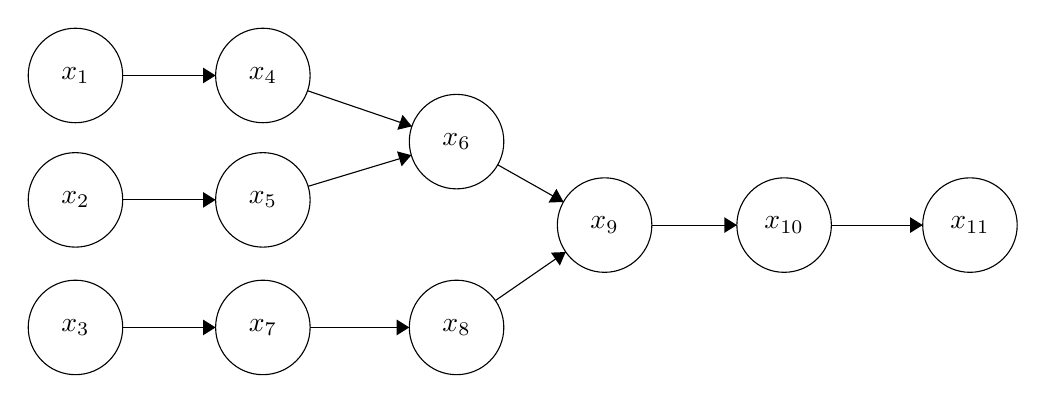
\begin{tikzpicture}[scale=0.2]
        \tikzstyle{every node}+=[inner sep=0pt]
        \draw [black] (4.9,-22.3) circle (3);
        \draw (4.9,-22.3) node {$x_1$};
        \draw [black] (4.9,-30.2) circle (3);
        \draw (4.9,-30.2) node {$x_2$};
        \draw [black] (16.8,-22.3) circle (3);
        \draw (16.8,-22.3) node {$x_4$};
        \draw [black] (16.8,-30.2) circle (3);
        \draw (16.8,-30.2) node {$x_5$};
        \draw [black] (29.1,-26.5) circle (3);
        \draw (29.1,-26.5) node {$x_6$};
        \draw [black] (4.9,-38.3) circle (3);
        \draw (4.9,-38.3) node {$x_3$};
        \draw [black] (16.8,-38.3) circle (3);
        \draw (16.8,-38.3) node {$x_7$};
        \draw [black] (29.1,-38.3) circle (3);
        \draw (29.1,-38.3) node {$x_8$};
        \draw [black] (38.5,-31.8) circle (3);
        \draw (38.5,-31.8) node {$x_9$};
        \draw [black] (49.9,-31.8) circle (3);
        \draw (49.9,-31.8) node {$x_{10}$};
        \draw [black] (61.7,-31.8) circle (3);
        \draw (61.7,-31.8) node {$x_{11}$};
        \draw [black] (7.9,-22.3) -- (13.8,-22.3);
        \fill [black] (13.8,-22.3) -- (13,-21.8) -- (13,-22.8);
        \draw [black] (7.9,-30.2) -- (13.8,-30.2);
        \fill [black] (13.8,-30.2) -- (13,-29.7) -- (13,-30.7);
        \draw [black] (19.64,-23.27) -- (26.26,-25.53);
        \fill [black] (26.26,-25.53) -- (25.67,-24.8) -- (25.34,-25.75);
        \draw [black] (19.67,-29.34) -- (26.23,-27.36);
        \fill [black] (26.23,-27.36) -- (25.32,-27.12) -- (25.61,-28.07);
        \draw [black] (7.9,-38.3) -- (13.8,-38.3);
        \fill [black] (13.8,-38.3) -- (13,-37.8) -- (13,-38.8);
        \draw [black] (19.8,-38.3) -- (26.1,-38.3);
        \fill [black] (26.1,-38.3) -- (25.3,-37.8) -- (25.3,-38.8);
        \draw [black] (31.57,-36.59) -- (36.03,-33.51);
        \fill [black] (36.03,-33.51) -- (35.09,-33.55) -- (35.66,-34.37);
        \draw [black] (31.71,-27.97) -- (35.89,-30.33);
        \fill [black] (35.89,-30.33) -- (35.44,-29.5) -- (34.94,-30.37);
        \draw [black] (41.5,-31.8) -- (46.9,-31.8);
        \fill [black] (46.9,-31.8) -- (46.1,-31.3) -- (46.1,-32.3);
        \draw [black] (52.9,-31.8) -- (58.7,-31.8);
        \fill [black] (58.7,-31.8) -- (57.9,-31.3) -- (57.9,-32.3);
        \end{tikzpicture}
    \end{center}
    where
    \begin{align*}
        x_4 &= x_1^2\\
        x_5 &= x_2^3\\
        x_7 &= x_3^4\\
        x_6 &= x_4\cdot x_5\\
        x_8 &= \sin(x_7)\\
        x_9 &= x_6+x_8\\
        x_{10} &= \exp(x_9)\\
        x_{11} &= x_{10}^2
    \end{align*}
    and we have the following derivatives
    \begin{align*}
        \frac{\partial x_4}{\partial x_1} &= 2x_1\\
        \frac{\partial x_5}{\partial x_2} &= 3x_2^2\\
        \frac{\partial x_7}{\partial x_3} &= 4x_3^3\\
        \frac{\partial x_6}{\partial x_4} &= x_5\\
        \frac{\partial x_6}{\partial x_5} &= x_4\\
        \frac{\partial x_8}{\partial x_7} &= \cos(x_7)\\
        \frac{\partial x_9}{\partial x_6} &= 1\\
        \frac{\partial x_9}{\partial x_8} &= 1\\
        \frac{\partial x_{10}}{\partial x_9} &= \exp(x_9)\\
        \frac{\partial x_{11}}{\partial x_{10}} &= 2x_{10}
    \end{align*}
    \begin{homeworkSubsection}{Forward Mode}
        We propogate the tangents through the computational graph 
        to compute the derivative of $f$ with respect to $x_1$, $x_2$ and $x_3$.
        Normally, we would have to propogate all the bases i.e. $\hat{i}$, $ \hat{j}$ and $ \hat{k}$ 
        one after another in order to all the partial derivatives
        but here each operation of the computational graph is a scalar operation
        and the starting node $x_1$, $x_2$ and $x_3$ are also scalas
        so we can simply set $\dot{x}_1 = 1$ when calculating $\frac{\partial f}{\partial x_1}$ and so on.
        To calculate the partial derivatives at point $(x_1, x_2, x_3) = (\tilde{x}_1, \tilde{x}_2, \tilde{x}_3)$, we have
        \begin{enumerate}
            \item[(i) $\frac{\partial f}{x_1}$]
            Set $\dot{x}_1 = 1, \dot{x}_2 = 0, \dot{x}_3 = 0$
            \begin{align*}
                x_1 &= \tilde{x}_1 & \dot{x}_1 &= 1\\
                x_2 &= \tilde{x}_2 & \dot{x}_2 &= 0\\
                x_3 &= \tilde{x}_3 & \dot{x}_3 &= 0\\
                x_4 &= x_1^2 = \tilde{x}_1^2 & \dot{x}_4 &= 2x_1\dot{x}_1 = 2\tilde{x}_1\dot{x}_1 = 2\tilde{x}_1\\
                x_5 &= x_2^3 = \tilde{x}_2^3 & \dot{x}_5 &= 3x_2^2\dot{x}_2 = 0\\
                x_6 &= x_4\cdot x_5 = \tilde{x}_1^2\cdot \tilde{x}_2^3 & \dot{x}_6 &= x_5\dot{x}_4 + x_4\dot{x}_5 = 2\tilde{x}_1\tilde{x}_2^3\\
                x_7 &= x_3^4 = \tilde{x}_3^4 & \dot{x}_7 &= 4x_3^3\dot{x}_3 = 0\\
                x_8 &= \sin(x_7) = \sin(\tilde{x}_3^4) & \dot{x}_8 &= \cos(x_7)\dot{x}_7 = 0\\
                x_9 &= x_6+x_8 = \tilde{x}_1^2\cdot \tilde{x}_2^3 + \sin(\tilde{x}_3^4) & \dot{x}_9 &= \dot{x}_6 + \dot{x}_8 = 2\tilde{x}_1\tilde{x}_2^3\\
                x_{10} &= \exp(x_9) = \exp(\tilde{x}_1^2\cdot \tilde{x}_2^3 + \sin(\tilde{x}_3^4)) & \dot{x}_{10} &= \exp(x_9)\dot{x}_9 = 2\exp(\tilde{x}_1^2\cdot \tilde{x}_2^3 + \sin(\tilde{x}_3^4))\tilde{x}_1\tilde{x}_2^3\\
                x_{11} &= x_{10}^2 = \exp(2(\tilde{x}_1^2\cdot \tilde{x}_2^3 + \sin(\tilde{x}_3^4))) & \dot{x}_{11} &= 2x_{10}\dot{x}_{10} = 4\exp(2(\tilde{x}_1^2\cdot \tilde{x}_2^3 + \sin(\tilde{x}_3^4)))\tilde{x}_1\tilde{x}_2^3
            \end{align*}
            \item[(ii) $\frac{\partial f}{x_2}$]
            Set $\dot{x}_1 = 0, \dot{x}_2 = 1, \dot{x}_3 = 0$.
            Repeat the same process as above we get
            \begin{align*}
                \frac{\partial f}{\partial x_2} &= 6\tilde{x}_1^2\tilde{x}_2^2\exp(2(\tilde{x}_1^2\cdot \tilde{x}_2^3 + \sin(\tilde{x}_3^4)))
            \end{align*}
            \item[(iii) $\frac{\partial f}{x_3}$]
            Set $\dot{x}_1 = 0, \dot{x}_2 = 0, \dot{x}_3 = 1$.
            Repeat the same process as above we get
            \begin{align*}
                \frac{\partial f}{\partial x_3} &= 8\tilde{x}_3^3\cos(\tilde{x}_3^4)\exp(2(\tilde{x}_1^2\cdot \tilde{x}_2^3 + \sin(\tilde{x}_3^4)))
            \end{align*}
        \end{enumerate}
    \end{homeworkSubsection}
    \begin{homeworkSubsection}{Backward Mode}
        We propogate normal vector of the hyperplane defined by $\langle\bar{y}, \nabla F(x)\rangle = c$ backward through the computational graph
        where $\bar{y}$ is the desired variation of the function $F$.
        For each partial derivatives, we set the normal vector to be the corresponding basis vector, i.e. $\bar{y} = \hat{i}$ for $\frac{\partial f}{\partial x_1}$ and so on.
        \begin{enumerate}
            \item [(i) $\frac{\partial f}{x_1}$]
            \begin{align*}
                x_1 &= \tilde{x}_1 & \\
                x_2 &= \tilde{x}_2 & \\
                x_3 &= \tilde{x}_3 & \\
                x_4 &= \tilde{x}_1^2 & \\
                x_5 &= \tilde{x}_2^3 & \\
                x_6 &= \tilde{x}_1^2\cdot \tilde{x}_2^3 & \\
                x_7 &= \tilde{x}_3^4 & \\
                x_8 &= \sin(\tilde{x}_3^4) & \\
                x_9 &= \tilde{x}_1^2\cdot \tilde{x}_2^3 + \sin(\tilde{x}_3^4) & \\
                x_{10} &= \exp(\tilde{x}_1^2\cdot \tilde{x}_2^3 + \sin(\tilde{x}_3^4)) & \\
                x_{11} &= \exp(2(\tilde{x}_1^2\cdot \tilde{x}_2^3 + \sin(\tilde{x}_3^4))) &\\
                && \bar{x}_{11} &= 1\\
                && \bar{x}_{10} &= 2\exp(\tilde{x}_1^2\cdot \tilde{x}_2^3 + \sin(\tilde{x}_3^4))\\
                && \bar{x}_9 &= 2\exp(2\tilde{x}_1^2\cdot \tilde{x}_2^3 + \sin(\tilde{x}_3^4))\\
                && \bar{x}_6 &= 2\exp(2\tilde{x}_1^2\cdot \tilde{x}_2^3 + \sin(\tilde{x}_3^4))\\
                && \bar{x}_4 &= 2\tilde{x}_2^3 \exp(2\tilde{x}_1^2\cdot \tilde{x}_2^3 + \sin(\tilde{x}_3^4))\\
                && \bar{x}_1 &= 4\tilde{x}_1\tilde{x}_2^3 \exp(2\tilde{x}_1^2\cdot \tilde{x}_2^3 + \sin(\tilde{x}_3^4))\\
            \end{align*}
        \end{enumerate}
        Similarly we can calculate the other partial derivatives. The result is the same as the forward mode.
    \end{homeworkSubsection}
\end{homeworkProblem}
\begin{homeworkProblem}[2]
    \begin{homeworkSubsection}{(a)}
        We construct a matrix $\tilde{P}_j$ for each column $j$ of $P$ such that 
        $\tilde{P}_j \in \mathbb{R}^{2\times 6}$
        \[
            \tilde{P}_j := \begin{pmatrix}
                P_{1j} & 0 & P_{2j} & 0 & 1 & 0\\
                0 & P_{1j} & 0 & P_{2j} & 0 & 1
            \end{pmatrix}
        \] 
        and we have $\tilde{P} \in \mathbb{R}^{2n\times 6}$ as following
        \[
            \tilde{P} := \begin{pmatrix}
                \tilde{P}_1\\
                \vdots\\
                \tilde{P}_n
            \end{pmatrix}
        \]
        At last, we construct $\tilde{Q} \in \mathbb{R}^{2n\times 1}$:
        \[
            \tilde{Q} := \begin{pmatrix}
                Q_1\\
                \vdots\\
                Q_n
            \end{pmatrix}
        \]
        where $Q_j$ denotes the $j$-th column of $Q$.
    \end{homeworkSubsection}
    \begin{homeworkSubsection}{(b)}
        The linear least squares problem can be formulated as
        \[
            \min_{x\in\mathbb{R}^3} \frac{1}{2}\norm{F(P, Q)}^2
        \]
        where 
        \[
            x:= \begin{pmatrix}
                t_1\\
                t_2\\
                \theta
            \end{pmatrix}
            \quad
            F(P, Q) := \tilde{P}A(x) - \tilde{Q}
        \] with $\tilde{P}$ and $\tilde{Q}$ defined in (a).
        
        The linear system of equations that need to be solved is 
        \[
            \nabla F(x^{(k)})\nabla F(x^{(k)})^\top d^{(k)} = - \nabla F(x^{(k)})F(x^{(k)})
        \]
        in order to calculate the descent direction $d^{(k)}$.
        $\nabla F(x^{(k)})$ can be calculated analytically. 
        It can also be approximated by finite difference.
    \end{homeworkSubsection}
\end{homeworkProblem}
\end{document}